\chapter{Lezione 3 - Enterprise Resource Planning System}

Benvenuti a questa nuova lezione sui sistemi per la gestione delle risorse d'impresa, Enterprise Resource Planning System.

Gli argomenti che tratteremo in questa lezione riguardano una descrizione dei sistemi, le varie funzionalità che devono sostenere, una visione di insieme di questi sistemi, di questi gruppi di funzionalità.

Argomenti trattati:

\FloatBarrier
\begin{figure}[H]
  \centering
  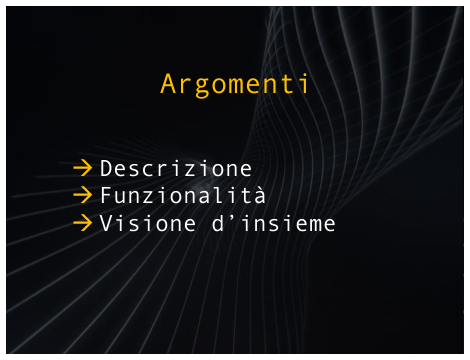
\includegraphics[width=0.50\textwidth,
                    trim=40 120 40 60, % L B R T
                    clip]
                    {images/Lez03_p01_fig_02}
  % \caption{Sommario}
  % \label{fig:Lez15_p06_fig_02}
\end{figure}
\FloatBarrier
\noindent

Cominciamo dalla descrizione.
Cosa sono questi sistemi per la gestione delle risorse d'impresa?

\FloatBarrier
\begin{figure}[H]
  \centering
  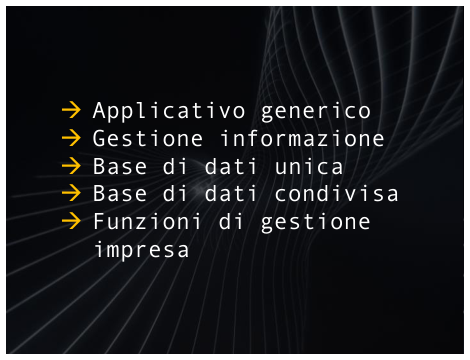
\includegraphics[width=0.50\textwidth,
                    trim=40 80 40 80, % L B R T
                    clip]
                    {images/Lez03_p01_fig_04}
  % \caption{Sommario}
  % \label{fig:Lez15_p06_fig_02}
\end{figure}
\FloatBarrier
\noindent

Sono innanzitutto degli applicativi generici.
Applicativo generico vuol dire che questi sistemi sono basati su una piattaforma, su una software applicativo generale che viene configurato sulla base delle necessità della singola impresa.
Questo vuol dire che l'insieme delle funzionalità che vengono soddisfatte con altrettanti gruppi di moduli software vengono scelti e raggruppati a costituire lo specifico Enterprise Resource Planning per quella data impresa.
Questi applicativi generici hanno come obiettivo principale la gestione delle informazioni.
La gestione delle informazioni è uno degli aspetti principali in un'impresa.
Perché?
Perché le informazioni devono essere uniche, quindi un dato deve correspondere, un'informazione deve essere sostenuta, deve essere misurata da un solo dato in qualunque sua versione e qualunque sua collocazione nell'ambito dei vari archivi di una di un'impresa.
Tutti i reparti dell'impresa devono disporre di informazioni analoghe, delle stesse informazioni, le informazioni devono essere quindi robuste e non ridondanti, quindi non ripetute.
Per questo vedremo che la gestione dell'informazione richiede determinate caratteristiche e deve soddisfare determinati principi che diano la rilevanza che merita a questo aspetto.

La base di dati, infatti, su cui si basano questi sistemi deve essere unica, in genere centralizzata o costituita da archivi distribuiti, ma con un controllo centrale o distribuita con una unicità di schema e di gestione di questi sistemi.

La base dei dati del sistema è condivisa, tutti i moduli, tutti i reparti, tutte le interfacce che vedremo costituiscono gli strumenti per l'interattività tra i vari dipendenti dell'impresa, devono poter accedere a questa base di dati.

Inoltre, tutte le funzioni di gestione dell'impresa potranno accedere a queste informazioni e coordinarsi, quindi offrire una alta interoperabilità che indica che le varie funzioni, i vari moduli possono da un lato comunicare tra di essi e dall'altro poter scambiare informazioni.

\FloatBarrier
\begin{figure}[H]
  \centering
  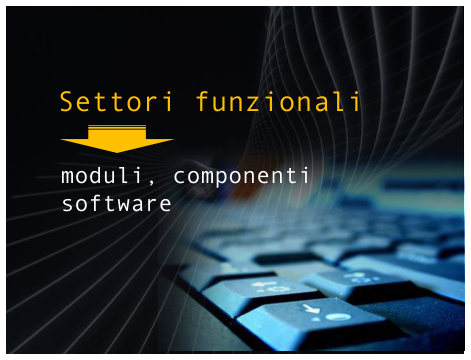
\includegraphics[width=0.50\textwidth,
                    trim=40 120 40 80, % L B R T
                    clip]
                    {images/Lez03_p01_fig_05}
  % \caption{Sommario}
  % \label{fig:Lez15_p06_fig_02}
\end{figure}
\FloatBarrier
\noindent


I vari settori funzionali di questi sistemi sono sostenuti da moduli, componenti software, che permettono la realizzazione, lo svolgimento opportuno, adeguato per gli scopi dell'impresa.

\subsection{Funzionalità}

Ma vediamo quali sono queste funzionalità, almeno quali sono le funzionalità principali che questi sistemi devono sostenere.

\FloatBarrier
\begin{figure}[H]
  \centering
  
\includegraphics[width=0.50\textwidth,
                    trim=40 120 40 80, % L B R T
                    clip]
                    {images/Lez03_p02_fig_01}
  % \caption{Sommario}
  % \label{fig:Lez15_p06_fig_02}
\end{figure}
\FloatBarrier
\noindent


Innanzitutto la contabilità.
Contabilità finanziaria e gestionale, quindi devono permettere la gestione del bilancio.
La gestione del bilancio indica sia la produzione, quindi disporre, attingere ai dati di base, ai dati sugli acquisti, sulle spese, sui costi del personale, ma anche la produzione, quindi le somme, tutte le operazioni amministrative che servono per la costruzione di un bilancio, e la reportistica, le statistiche che accompagnano la presentazione di un bilancio.

Quindi saranno necessarie anche funzioni per la gestione dei costi di tutti i costi che riguardano l'impresa, che toccheranno quindi vari settori, dal settore commerciale, quindi la gestione dei costi dei prodotti acquisiti, ma anche la gestione del personale, quindi i costi del personale sia come stipendi, sia anche come costi di struttura per le spese condominiali, i consumi di energia, piuttosto che i viaggi, piuttosto che l'ambito, l'ufficio in cui svolgono le proprie attività.

I costi delle singole attività, quindi sia le attività interne ma sia anche i costi per attività commissionate in outsourcing, commissionate a consulenze esterni o eventuali verifiche da far effettuare sulla impresa.

\FloatBarrier
\begin{figure}[H]
  \centering
  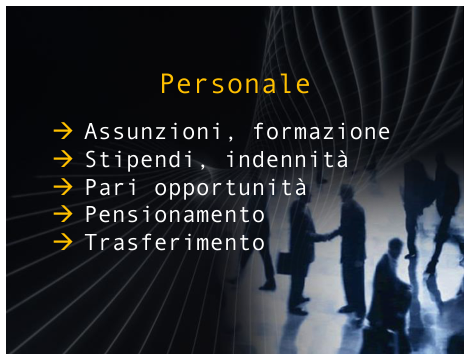
\includegraphics[width=0.50\textwidth,
                    trim=40 90 40 60, % L B R T
                    clip]
                    {images/Lez03_p02_fig_02}
  % \caption{Sommario}
  % \label{fig:Lez15_p06_fig_02}
\end{figure}
\FloatBarrier
\noindent

Il gruppo cruciale, il gruppo basilare  di un'impresa è il gruppo di attività che riguarda il gruppo di funzionalità che riguardano il personale, sia per la gestione della pianta organica, quindi sia le assunzioni, quindi il personale in carico, lo stato del personale presente, assente, assunto a tempo determinato, sia anche la formazione del personale.
Per formazione del personale intendiamo proprio seguire, archiviare, tracciare il percorso di crescita del personale che è stato acquisito o che collabora allo svolgimento delle attività dell'impresa.

Gli stipendi dicevamo, l'indennità, quindi i costi diretti del personale, i costi che vengono forniti, che vengono pagati al personale per i costi netti, i costi che vengono erogati al personale per lo svolgimento delle proprie attività.

Questioni che riguardano le pare opportunità, quindi questioni di genere, ma anche questioni di uguaglianza sul lavoro, questioni etiche, questioni riguardanti non tanto gli aspetti sindacali, quanto gli aspetti proprio di uguaglianza rispetto alle normative di presenza e di svolgimento delle attività lavorative.

I pensionamenti sia per pianificare l'acquisizione di nuove risorse, giovani risorse da crescere all'interno dell'impresa, sia anche per pianificare la presenza o misurare meglio la presenza del personale, le risorse umane dell'impresa da qui a un breve periodo di tempo, sia per i costi di uscita del personale, sia anche per poter pianificare attività sulla base delle persone che saranno nell'impresa tra uno, due o tre anni.

Allo stesso tempo bisognerà misurare quelle che sono le variazioni forse più in inattese ma nel breve termine meno misurabili dei cambiamenti di quantità di risorse personali dovute al pensionamento, quindi i trasferimenti, sia tra gli stessi reparti di un'impresa per un cambio di funzione, sia anche per movimenti ad altre sedi, ad altre succursali agenzie della stessa organizzazione, sia anche per dimissioni, per assunzioni in altre imprese, proprio un cambio di attività lavorativa.

\FloatBarrier
\begin{figure}[H]
  \centering
  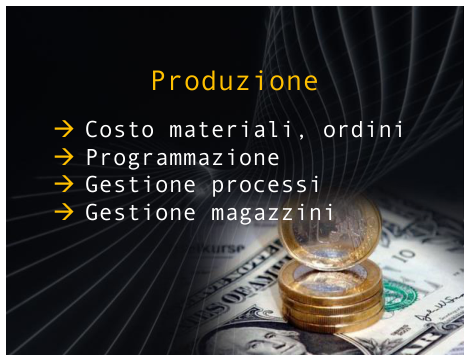
\includegraphics[width=0.50\textwidth,
                    trim=40 120 40 50, % L B R T
                    clip]
                    {images/Lez03_p02_fig_03}
  % \caption{Sommario}
  % \label{fig:Lez15_p06_fig_02}
\end{figure}
\FloatBarrier
\noindent

Un altro settore di funzionalità è il settore della produzione che inizia con l'acquisizione dei materiali degli ordini, quindi un'attività che rientra in qualche modo, che si sovrappone alle attività di gestione finanziaria o di gestione finanziaria commerciale che riguarda l'acquisizione dei materiali, quindi gli ordini che sono stati arrogati, quindi si suppone che i materiali richiesti per lo svolgimento delle varie attività siano a questo punto immagazzinati nell'impresa, quindi disponibili per lo svolgimento delle attività, sia i materiali che sono stati previsti ma non sono ancora arrivati per eventuali solleciti, per attivare quindi automaticamente o allertare il back office dell'impresa di richiedere, sollecitare lo smaltimento di questi ordini, quindi l'arrivo dei nuovi prodotti, delle nuove risorse necessarie, sia anche per poter misurare le risorse che non sono ancora state ordinate ma che sono necessarie e devono essere previste per lo svolgimento futuro delle attività.

Quindi è necessaria la programmazione per i motivi che discutevamo per poter non semplicemente avere l'immagine istantanea dell'oggi, le risorse che sono disponibili, le risorse di cui avremo bisogno ma poter avere una visione sull'ordinato, quello che deve arrivare e su quanto e cosa è il caso di pianificare e di ordinare per le attività future, quindi proprio un'attività di programma futuro.

Nella produzione è necessaria la gestione dei processi, proprio come processi lavorativi, come workflow, quindi proprio lo svolgimento delle attività con le risorse, attraverso le risorse disponibili, il passaggio delle risorse elaborate alle successive attività, attraverso l'intervento o meglio l'interattività delle varie risorse umane, delle varie persone, dei vari lavoratori dell'impresa.

Inoltre, o diciamo, per quanto riguarda le scorte di risorse materiali, la gestione dei magazzini.
La gestione dei magazzini serve proprio per poter misurare la durata nel breve o nel medio periodo delle attività sulla base delle risorse attualmente disponibili, delle risorse i cui ordini sono già stati smaltiti e le forniture sono state erogate.

\FloatBarrier
\begin{figure}[H]
  \centering
  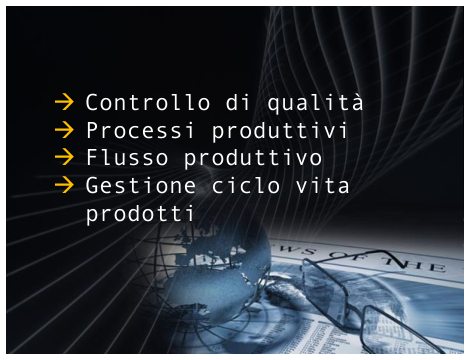
\includegraphics[width=0.50\textwidth,
                    trim=40 120 40 80, % L B R T
                    clip]
                    {images/Lez03_p02_fig_04}
  % \caption{Sommario}
  % \label{fig:Lez15_p06_fig_02}
\end{figure}
\FloatBarrier
\noindent

Il controllo della qualità.
Il controllo della qualità è la verifica che le attività di un'impresa siano soggette a una normativa ufficiale, da una normativa consolidata o accettata, una normativa di riferimento.
Vengono definite da queste normative sia le modalità di svolgimento delle attività, sia tutta la documentazione che deve essere svolta, mantenuta durante lo svolgimento di queste attività.
La documentazione sia per la verifica di come si sono svolte queste attività dagli eventuali audit, dagli eventuali valutatori, sia anche la documentazione che deve essere fornita alle generazioni future, alle nuove generazioni, alle nuove acquisizioni di risorse di personali, sia anche per la documentazione, la informazione tra i vari reparti dell'impresa.

Queste informazioni, queste documentazioni servono per la gestione dei processi produttivi, gestione dei processi produttivi anche o forse soprattutto per quanto riguarda non solo, come dicevamo, la gestione delle risorse, ma anche proprio il flusso produttivo.
Il flusso produttivo, quindi lo svolgimento delle singole attività, non solo per quanto riguarda le risorse, i costi, l'energia funzionale che deve essere, l'energia delle persone che deve essere erogata, ma anche proprio la correttezza temporale di svolgimento delle varie attività.

Tutte queste attività devono garantire la gestione del ciclo di vita dei prodotti, quindi il controllo della qualità del flusso, del ciclo di svolgimento delle attività e delle risorse di modalità di acquisizione, di mantenimento ed erogazione delle varie risorse che sono utilizzate e necessarie per lo svolgimento delle attività dell'impresa.

\FloatBarrier
\begin{figure}[H]
  \centering
  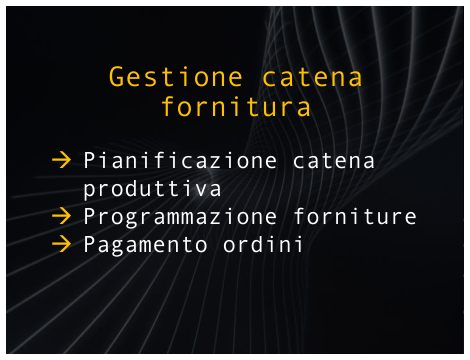
\includegraphics[width=0.50\textwidth,
                    trim=40 80 40 60, % L B R T
                    clip]
                    {images/Lez03_p02_fig_05}
  % \caption{Sommario}
  % \label{fig:Lez15_p06_fig_02}
\end{figure}
\FloatBarrier
\noindent

Passiamo ora alla gestione della catena di fornitura, quindi l'entrata delle risorse umane o materiali.
La pianificazione, la pianificazione quindi della catena produttiva, catena produttiva indica tutto l'insieme delle attività che vengono svolte in produzione.

Inoltre, come avevamo accennato, la programmazione delle forniture, delle forniture sia di risorse umane e di attività, sia anche di risorse materiali.

E la verifica del pagamento degli ordini.
Facciamo un attimo differenza, anche se è una sottile differenza, tra l'erogazione dell'ordine, tra la formulazione di un ordine, tra la manifestazione di dover erogare un ordine per acquisire delle risorse e la verifica, quindi un'operazione gestionale di verifica, che l'ordine sia stato smaltito.

\FloatBarrier
\begin{figure}[H]
  \centering
  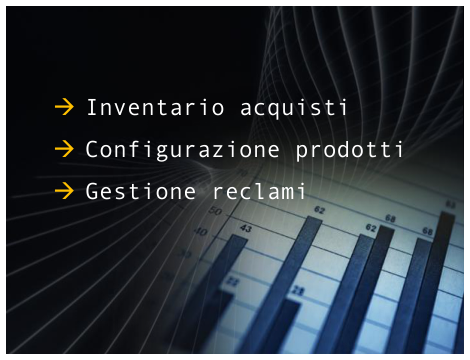
\includegraphics[width=0.50\textwidth,
                    trim=40 120 40 80, % L B R T
                    clip]
                    {images/Lez03_p02_fig_06}
  % \caption{Sommario}
  % \label{fig:Lez15_p06_fig_02}
\end{figure}
\FloatBarrier
\noindent

L'inventario degli acquisti.
Le scorte vengono immagazzinate quando entrano nell'impresa e l'inventario permette di avere una costante immagine, una costante configurazione della presenza delle risorse e del tipo delle risorse disponibili in un dato istante nell'impresa.

La configurazione dei prodotti sia in quantità, sia in qualità, sia in collocazione, quindi in quale magazzino sono stati archiviati, dove in un dato grande magazzino sono stati archiviati.

La gestione dei reclami.
Riguarda il tratto finale, se vogliamo, o la fase finale del prodotto, quando il prodotto è stato affidato, è stato passato al cliente, è stato acquistato, ma possono intervenire reclami piuttosto che richieste di aggiornamento, richieste di modifica o, più semplicemente o più ottimisticamente, richieste di manutenzione dei prodotti o dei servizi che sono forniti.

\FloatBarrier
\begin{figure}[H]
  \centering
  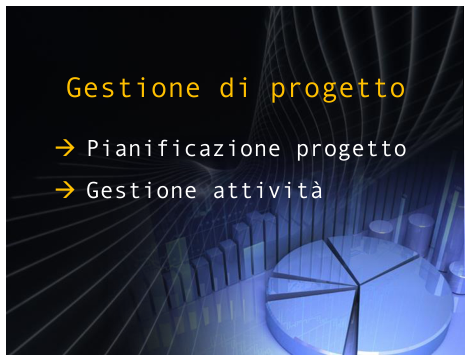
\includegraphics[width=0.50\textwidth,
                    trim=40 120 40 60, % L B R T
                    clip]
                    {images/Lez03_p03_fig_01}
  % \caption{Sommario}
  % \label{fig:Lez15_p06_fig_02}
\end{figure}
\FloatBarrier
\noindent

Gestione del progetto.
Il progetto, un progetto di impresa che è sostenuto con l'attività e con le risorse, deve essere innanzitutto pianificato.
La pianificazione del prodotto riguarda la misurazione, la scelta dell'attività e delle risorse e la quantificazione della loro necessità per il corretto svolgimento e efficace, quindi per il poter portare a termine, per poter concludere il progetto.
Quindi la gestione dell'attività.

\FloatBarrier
\begin{figure}[H]
  \centering
  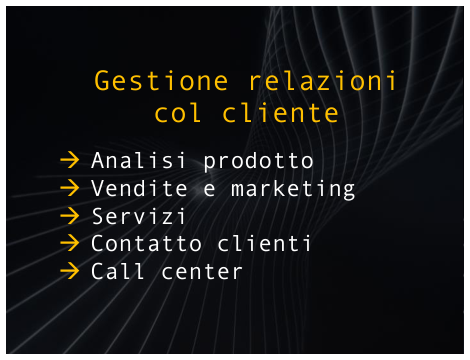
\includegraphics[width=0.50\textwidth,
                    trim=40 60 40 60, % L B R T
                    clip]
                    {images/Lez03_p03_fig_02}
  % \caption{Sommario}
  % \label{fig:Lez15_p06_fig_02}
\end{figure}
\FloatBarrier
\noindent

La fase di gestione delle relazioni col cliente è una fase che copre sia la parte iniziale del ciclo di vita di un prodotto, quindi la fase di marketing, la fase di indagine delle necessità di utente per poter creare prodotti giusti, ma sia anche una considerazione del feedback per poter quindi rianalizzare il prodotto.

Quindi i due aspetti, le vendite e il marketing, la fine del prodotto ma anche l'inizio o l'aggiornamento per produrre nuovi prodotti.

La gestione delle relazioni col cliente riguarda anche i servizi che può essere necessario svolgere per il cliente.
Servizi di informazione, quindi discussione sui prodotti venduti, ma anche contributi, raccolte di feedback per poter continuare il legame, fidelizzare i clienti e anche poter modificare le nuove versioni, le nuove generazioni dei prodotti.

Naturalmente la gestione del contatto con i clienti è una attività specifica.
Attualmente specie nelle realtà con grandi quantità di clienti o attività che richiedono una grande interazione  dell'azienda, del back office con i clienti, i servizi di contatto col clienti sono svolti da uffici specifici.
L'ufficio contatto acquisirà poi o verrà sostenuto da uffici specifici per questioni tecniche piuttosto che questioni di manutenzione e piuttosto che questioni commerciali per eventuali scambi del prodotto.
Questi uffici di contatto, questi servizi di contatto sono svolti dai ormai famosi, molto diffusi call center, che sono proprio centri dedicati alla raccolta, alla gestione della comunicazione, ma alla raccolta delle informazioni, dei dati provenienti per il cliente.

\FloatBarrier
\begin{figure}[H]
  \centering
  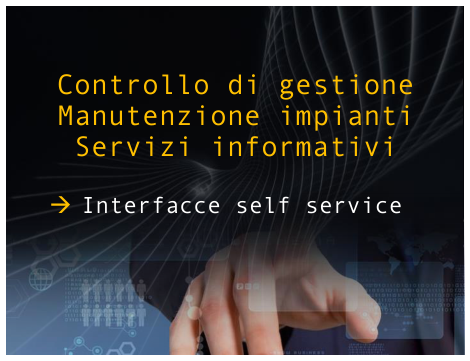
\includegraphics[width=0.50\textwidth,
                    trim=40 60 40 60, % L B R T
                    clip]
                    {images/Lez03_p03_fig_03}
  % \caption{Sommario}
  % \label{fig:Lez15_p06_fig_02}
\end{figure}
\FloatBarrier
\noindent


Questi tre servizi li mostriamo insieme, sono servizi orizzontali, controllo di gestione, manutenzione degli impianti e servizi informativi trasversali che sostengono tutti i moduli, tutti quindi i servizi che sostengono le funzionalità di un'impresa.

\FloatBarrier
\begin{figure}[H]
  \centering
  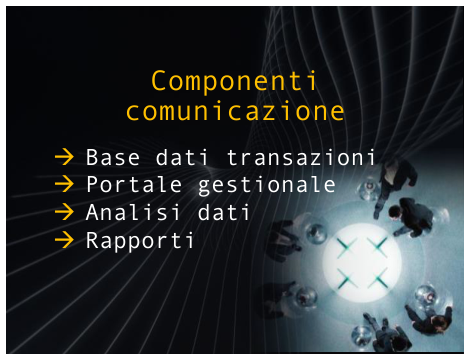
\includegraphics[width=0.50\textwidth,
                    trim=40 80 40 60, % L B R T
                    clip]
                    {images/Lez03_p03_fig_04}
  % \caption{Sommario}
  % \label{fig:Lez15_p06_fig_02}
\end{figure}
\FloatBarrier
\noindent

Un discorso dedicato va fatto alle componenti di comunicazione.
Le componenti di comunicazione sono rilevanti sia per l'interattività dei dipendenti di un'organizzazione, sia anche per i rapporti con il cliente.
Sono basati su sistemi per la gestione delle transazioni, il movimento dei dati, sia verso l'esterno, sia verso l'interno, ma sia anche all'interno tra i vari dipendenti.

Sono basati tipicamente, almeno nelle nuove generazioni di comunicazione, sul portale gestionale, un'applicazione web che serve da una parte a fornire informazioni all'esterno, presentare il prodotto, propagandare il prodotto, d'altro lato offre anche servizi di community, servizi di comunicazione per raccogliere i feedback, per mandare richieste, quindi possibili caselle di posta elettronica, forum di discussione e quant'altro possa essere necessario, utile per la comunicazione, per il rapporto con i clienti, ma anche nel caso di sezioni protette, sezioni di intranet del portale, per lo scambio di informazioni e l'interattività all'interno dell'organizzazione, quindi un sistema di supporto per le attività di back office.

L'analisi dei dati che vengono raccolti è un'attività molto importante per le imprese, sia per le future attività di marketing, sia anche per la definizione più a lungo termine delle strategie di impresa e per la produzione dei rapporti di documentazione o presentazione delle attività svolte.

\FloatBarrier
\begin{figure}[H]
  \centering
  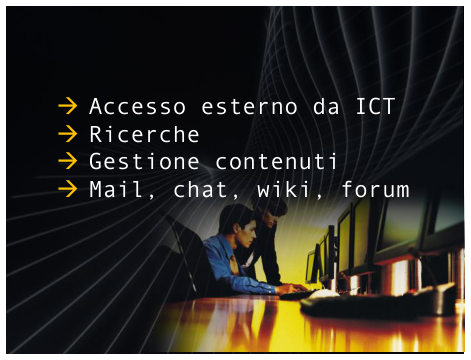
\includegraphics[width=0.50\textwidth,
                    trim=40 120 40 60, % L B R T
                    clip]
                    {images/Lez03_p03_fig_05}
  % \caption{Sommario}
  % \label{fig:Lez15_p06_fig_02}
\end{figure}
\FloatBarrier
\noindent

E' pure possibile sostenuti dalle moderne tecnologie di information communication technologies di accedere a servizi esterni all'impresa, quindi avere l'applicazione generica e il nostro enterprise resource planning che utilizza le attività realizzate da moduli, servizi, software offerti da piattaforme remote.

Funzionalità importante, e anche in quest'ambito di tecnologie dell'informazione, sono gli strumenti per la ricerca dell'informazione, che siano crawler, che siano anche possibili accessi ad archivi non necessariamente gestiti dalla impresa stessa.

Sistemi di gestione dei contenuti, con un'accezione più generale, non solo di documenti, ma più focalizzata all'aspetto semantico, all'argomento, al senso che viene dato con testi, messaggi, piuttosto che contributi in forum.
Quello che interessa ai sistemi di gestione dei contenuti è proprio l'argomento che viene trattato.

Ma anche, più semplicemente per la comunicazione, quello che è lo scambio, la messaggistica, quindi scambio di messaggi asincroni, nel tempo, sincroni, quindi per messageria istantanea, sistemi wiki per la produzione di documenti in maniera collaborativa a più mani, quindi a più contributi, o forum, per discussioni approfondite su problemi, su soluzioni, su nuove iniziative.

A questo punto, alla fine di quest'argomento, vi propongo due spunti di riflessione.
Provate a descrivere l'ambito professionale o formativo a cui avete accesso.
Quindi, se avete una vostra attività svolta in un ambito lavorativo, oppure se preferite scegliere l'ambito formativo universitario che frequentate.
Descritto quest'ambito, provate a descrivere le funzionalità, immaginare le funzionalità di un enterprise resource planning (ERPS) a supporto di questo ambito.

\section{Visione d'insieme}

\FloatBarrier
\begin{figure}[H]
  \centering
  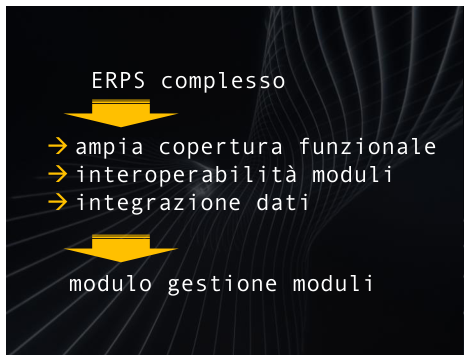
\includegraphics[width=0.50\textwidth,
                    trim=40 40 40 60, % L B R T
                    clip]
                    {images/Lez03_p04_fig_03}
  % \caption{Sommario}
  % \label{fig:Lez15_p06_fig_02}
\end{figure}
\FloatBarrier
\noindent


Vediamo ora una visione d'insieme del sistema composto da questo grande insieme di funzionalità che abbiamo visto.
Ci siamo resi conto che l'enterprise resource planning è un sistema complesso che fornisce un'ampia copertura funzionale, quindi offre strumenti eterogenei diversi che permettono di svolgere diverse funzioni, offrire diversi servizi necessari alla conduzione di un'azienda, alla conduzione delle diverse attività che vengono svolte dai diversi reparti che compongono una qualsiasi organizzazione aziendale.

La diversità di questi moduli, la diversità dei reparti, delle necessità e delle funzionalità richieste richiede un'alta interoperabilità tra i vari moduli.
Interoperabilità sia per lo scambio dei dati, quindi interoperabilità sintatica, ma anche interoperabilità perché non ci dovrebbe essere soluzione di continuità tra le attività svolte da un modulo e le attività svolte dall'altro.
Cioè i moduli non dovrebbero avere nessun problema a svolgere parti di un'attività più complessa.

Il terzo punto è l'integrazione dei dati.
Le informazioni e i dati che le costituiscono svolgono un ruolo molto importante per la conduzione, per la buona gestione del sistema, per la gestione delle risorse di impresa.
Le informazioni devono essere pure loro ben gestite, ma questa complessità viene attualmente spesso gestita da uno specifico modulo di gestione, un modulo supervisore, un modulo per la gestione degli altri moduli specialistici.

Noi abbiamo due tipi di gestione integrata in un sistema complesso.
Specificatamente, noi lo vedremo nelle prossime slide per quanto riguarda ovviamente il sistema per la gestione delle risorse di impresa.

\FloatBarrier
\begin{figure}[H]
  \centering
  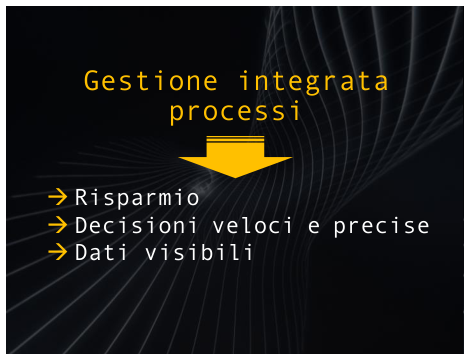
\includegraphics[width=0.50\textwidth,
                    trim=40 60 40 60, % L B R T
                    clip]
                    {images/Lez03_p04_fig_04}
  % \caption{Sommario}
  % \label{fig:Lez15_p06_fig_02}
\end{figure}
\FloatBarrier
\noindent

Sono la gestione integrata dei processi per un maggiore risparmio, per poter prendere decisioni veloci e precise e per offrire dati che siano visibili in tutta la realtà aziendale.
Ed eventualmente, come abbiamo visto, nel caso di fidelizzazione, nel caso di gestione dei rapporti col cliente, anche all'esterno dell'impresa.
Ecco, la gestione integrata dei processi serve per dare solidità a questi tre obiettivi, a queste tre necessità del buon funzionamento di un'impresa.

\FloatBarrier
\begin{figure}[H]
  \centering
  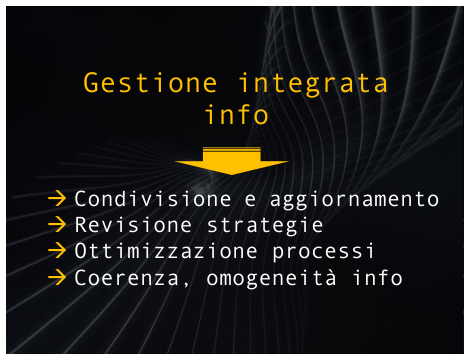
\includegraphics[width=0.50\textwidth,
                    trim=40 60 40 60, % L B R T
                    clip]
                    {images/Lez03_p04_fig_05}
  % \caption{Sommario}
  % \label{fig:Lez15_p06_fig_02}
\end{figure}
\FloatBarrier
\noindent

La gestione integrata delle informazioni porta o richiede la condivisione e l'aggiornamento delle informazioni, delle basi informative.

Permette una revisione delle strategie fornendo dati aggiornati, robusti e di prospettiva.

Permette di ottimizzare i processi.
Tutti i processi fanno riferimento alla stessa base informativa, corretta, quindi permette una economia di gestione e permette anche di raccogliere i dati dove e quando servono.

Le informazioni ben gestite permettono una coerenza e un'omogeneità.

Le informazioni hanno un solo valore, non sono ridondanti e non forniscono o sono gestite le varie versioni degli stessi dati, delle stesse informazioni, degli stessi documenti nell'ambito del sistema informativo distribuito dell'impresa.

\FloatBarrier
\begin{figure}[H]
  \centering
  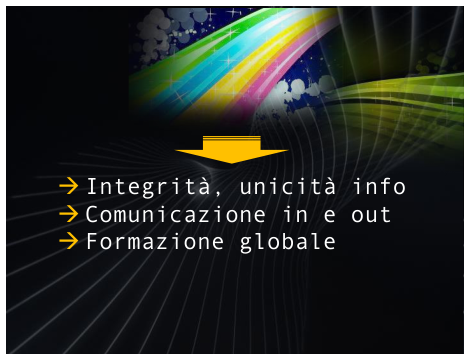
\includegraphics[width=0.50\textwidth,
                    trim=40 80 40 60, % L B R T
                    clip]
                    {images/Lez03_p04_fig_06}
  % \caption{Sommario}
  % \label{fig:Lez15_p06_fig_02}
\end{figure}
\FloatBarrier
\noindent

Una buona gestione delle informazioni fornisce l'integrità e l'unicità dell'informazione, ma anche quindi sostiene la comunicazione all'interno e verso l'esterno dell'organizzazione e una formazione globale.
Formazione globale che è riferita o che è sostenuta dalla possibilità di accesso alle informazioni uniche e riservate dell'impresa, alla documentazione, a tutto il materiale che serve per addestrare le persone, per aggiornare le persone, le risorse umane che vengono acquisite dall'impresa.
%31:20

\FloatBarrier
\begin{figure}[H]
  \centering
  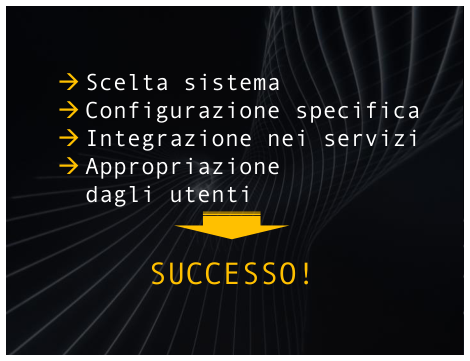
\includegraphics[width=0.50\textwidth,
                    trim=40 60 40 60, % L B R T
                    clip]
                    {images/Lez03_p05_fig_01}
  % \caption{Sommario}
  % \label{fig:Lez15_p06_fig_02}
\end{figure}
\FloatBarrier
\noindent

La scelta del sistema, la corretta scelta del sistema e per corretta mi riferisco al contesto aziendale, alle necessità dell'impresa.

Inoltre la configurazione specifica adatta a questa realtà, a questo contesto, l'integrazione nei servizi attualmente svolti, attualmente erogati e l'appropriazione da parte degli utenti sono le chiavi del successo dell'enterprise resource planning di un'impresa.

E per appropriazione degli utenti ci riferiamo sia agli utenti clienti, agli utenti customer, agli utenti esterni, sia anche agli utenti quali lavoratori nel back office dell'impresa.

\FloatBarrier
\begin{figure}[H]
  \centering
  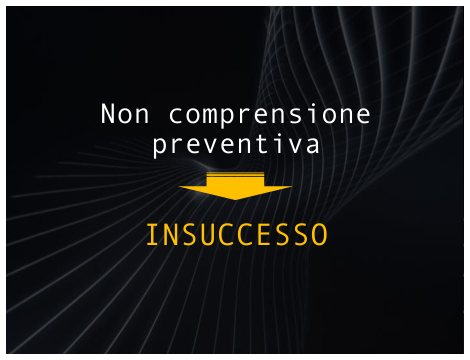
\includegraphics[width=0.50\textwidth,
                    trim=40 60 40 60, % L B R T
                    clip]
                    {images/Lez03_p05_fig_02}
  % \caption{Sommario}
  % \label{fig:Lez15_p06_fig_02}
\end{figure}
\FloatBarrier
\noindent

Il non comprendere preventivamente, correttamente nel dettaglio i servizi, le funzionalità e le necessità soprattutto, gli obiettivi a cui punta un'impresa, sono invece la chiave per l'insuccesso di un enterprise resource planning.

Vogliamo intendere che il successo di un sistema del genere complesso non sono nell'acquisizione di un moderno sistema tecnologico, ma nell'acquisizione del corretto moderno sistema tecnologico.

\FloatBarrier
\begin{figure}[H]
  \centering
  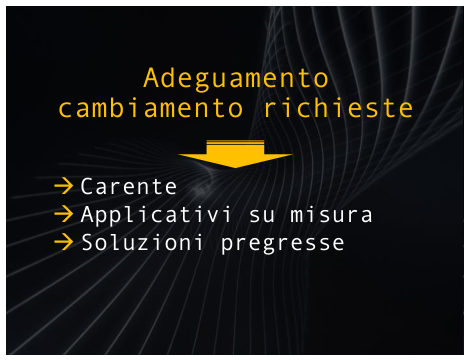
\includegraphics[width=0.50\textwidth,
                    trim=40 80 40 60, % L B R T
                    clip]
                    {images/Lez03_p05_fig_03}
  % \caption{Sommario}
  % \label{fig:Lez15_p06_fig_02}
\end{figure}
\FloatBarrier
\noindent

Un occhio adesso all'adeguamento, al cambiamento delle richieste.
Il sistema informativo è un sistema complesso che viene utilizzato per lunghi periodi in un'impresa.
Il cambiamento, l'adeguamento al cambiamento delle richieste è stato fino a poco tempo fa carente.
Carente perché soprattutto gli applicativi che servivano per lo svolgimento delle attività, venivano commissionati e implementati su misura basati spesso su soluzioni prodotte per risolvere problemi pregressi.

\FloatBarrier
\begin{figure}[H]
  \centering
  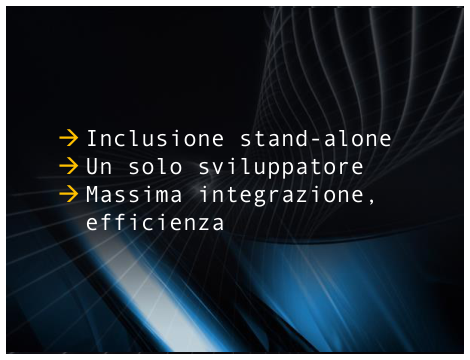
\includegraphics[width=0.50\textwidth,
                    trim=40 100 40 80, % L B R T
                    clip]
                    {images/Lez03_p05_fig_04}
  % \caption{Sommario}
  % \label{fig:Lez15_p06_fig_02}
\end{figure}
\FloatBarrier
\noindent


C'è stata un'evoluzione verso l'inclusione di soluzioni stand alone, sempre però risolte, implementate da un solo sviluppatore che fornisce la massima integrazione d'efficienza, che sono due valori sì positivi, ma che fanno perdere molto alla modularità, all'elasticità e all'estensibilità, all'aggiornamento e alla modificabilità di un sistema complesso.

\FloatBarrier
\begin{figure}[H]
  \centering
  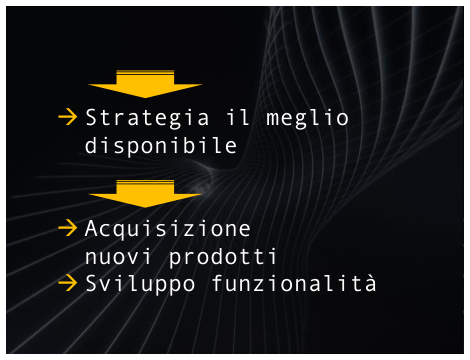
\includegraphics[width=0.50\textwidth,
                    trim=40 60 40 60, % L B R T
                    clip]
                    {images/Lez03_p05_fig_05}
  % \caption{Sommario}
  % \label{fig:Lez15_p06_fig_02}
\end{figure}
\FloatBarrier
\noindent

Nella seconda fase di sviluppo di questi sistemi si è passata a quella che viene chiamata strategia il meglio disponibile, cioè le soluzioni vengono prodotte acquisendo nuovi prodotti e sviluppando funzionalità che fossero però riferite al meglio disponibile sul mercato, quindi eventualmente sviluppate ancora da un singolo implementatore, ma che avesse come riferimento da una parte l'alta integrazione all'interno del sistema aziendale, ma con riferimento per gli aggiornamenti e le estensioni al meglio agli applicativi di punta disponibili in quel momento sul mercato.

\FloatBarrier
\begin{figure}[H]
  \centering
  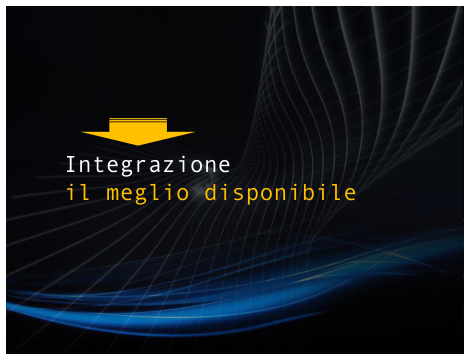
\includegraphics[width=0.50\textwidth,
                    trim=40 120 40 80, % L B R T
                    clip]
                    {images/Lez03_p05_fig_06}
  % \caption{Sommario}
  % \label{fig:Lez15_p06_fig_02}
\end{figure}
\FloatBarrier
\noindent

La terza fase di sviluppo per il buon aggiornamento di questi sistemi è la terza fase di integrazione del meglio disponibile.
L'integrazione del meglio disponibile si riferisce al fatto che non necessariamente i sistemi vengono implementati.
Noi abbiamo visto all'inizio che l'enterprise resouce planning è un servizio, è un sistema general purpose che viene esteso con applicativi, vediamo in questa nuova moderna metodologia di estensione e di aggiornamento del sistema che viene esteso acquisendo componenti migliori sul mercato.

\FloatBarrier
\begin{figure}[H]
  \centering
  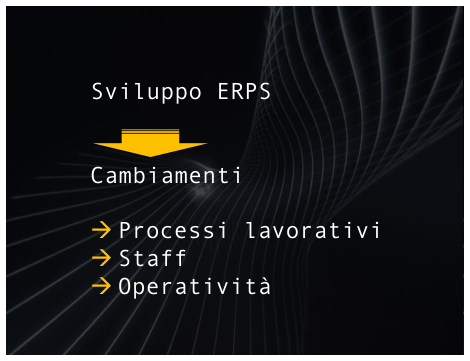
\includegraphics[width=0.50\textwidth,
                    trim=40 40 40 60, % L B R T
                    clip]
                    {images/Lez03_p06_fig_01}
  % \caption{Sommario}
  % \label{fig:Lez15_p06_fig_02}
\end{figure}
\FloatBarrier
\noindent

Lo sviluppo di un enterprise resource planning porta cambiamenti non solo nella gestione delle informazioni o dell'attività in senso della computer science, quindi automatico, tecnologico, ma anche dei processi lavorativi.
Devono essere aggiornati nel loro modo, ma anche nella figure funzionali necessari, le competenze disponibili e nell'operatività, quindi nello svolgimento effettivo delle attività svolte.

\FloatBarrier
\begin{figure}[H]
  \centering
  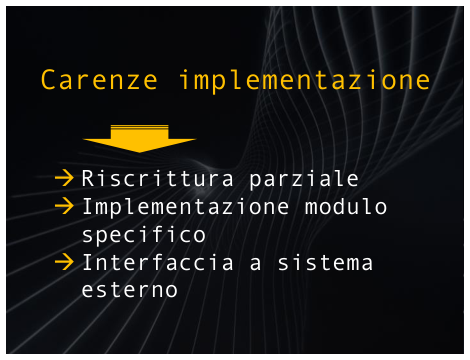
\includegraphics[width=0.50\textwidth,
                    trim=40 40 40 60, % L B R T
                    clip]
                    {images/Lez03_p06_fig_02}
  % \caption{Sommario}
  % \label{fig:Lez15_p06_fig_02}
\end{figure}
\FloatBarrier
\noindent

Le carenze dell'implementazione di un sistema informativo in senso generale nello specifico di un enterprise resource planning portano a una riscrittura parziale del codice o all'inclusione di nuovi moduli, all'implementazione di nuove specifiche funzioni o l'interfacciamento a sistemi esterni che, come abbiamo visto, possono essere interpellati per l'acquisizione di nuove funzionalità, eventualmente utilizzando le moderne tecnologie di web service che vedremo in altre lezioni.

\FloatBarrier
\begin{figure}[H]
  \centering
  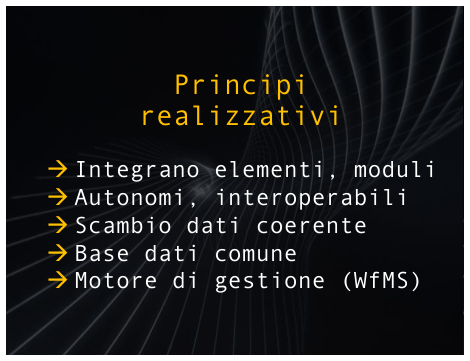
\includegraphics[width=0.50\textwidth,
                    trim=20 40 20 60, % L B R T
                    clip]
                    {images/Lez03_p06_fig_03}
  % \caption{Sommario}
  % \label{fig:Lez15_p06_fig_02}
\end{figure}
\FloatBarrier
\noindent

I principi realizzativi per questi sistemi sono l'integrazione, come abbiamo visto, di elementi o di moduli software che siano autonomi e interoperabili, sia sintaticamente sia anche semanticamente.
Lo scambio di dati è coerente, la base di dati, quindi comune e in genere deve essere o è utile che abbiano a disposizione un sistema per la gestione, un motore per la gestione dei workflow, dei flussi lavorativi.
In conclusione di questo argomento e di questa lezione vorrei proporvi due spunti di riflessione.
Supponete che sia cambiata la gestione del personale nella vostra organizzazione lavorativa o ancora formativa nella vostra università. Che interventi vi aspettate debbano essere portati sulle enterprise resource planning, che aggiornamenti, che estensioni o quali servizi, funzionalità non sono più necessarie.
Il secondo spunto è che scelte implementative erano state fatte invece per il suo sviluppo, commentate le differenze.

